% Options for packages loaded elsewhere
\PassOptionsToPackage{unicode}{hyperref}
\PassOptionsToPackage{hyphens}{url}
%
\documentclass[
]{article}
\usepackage{amsmath,amssymb}
\usepackage{lmodern}
\usepackage{ifxetex,ifluatex}
\ifnum 0\ifxetex 1\fi\ifluatex 1\fi=0 % if pdftex
  \usepackage[T1]{fontenc}
  \usepackage[utf8]{inputenc}
  \usepackage{textcomp} % provide euro and other symbols
\else % if luatex or xetex
  \usepackage{unicode-math}
  \defaultfontfeatures{Scale=MatchLowercase}
  \defaultfontfeatures[\rmfamily]{Ligatures=TeX,Scale=1}
\fi
% Use upquote if available, for straight quotes in verbatim environments
\IfFileExists{upquote.sty}{\usepackage{upquote}}{}
\IfFileExists{microtype.sty}{% use microtype if available
  \usepackage[]{microtype}
  \UseMicrotypeSet[protrusion]{basicmath} % disable protrusion for tt fonts
}{}
\makeatletter
\@ifundefined{KOMAClassName}{% if non-KOMA class
  \IfFileExists{parskip.sty}{%
    \usepackage{parskip}
  }{% else
    \setlength{\parindent}{0pt}
    \setlength{\parskip}{6pt plus 2pt minus 1pt}}
}{% if KOMA class
  \KOMAoptions{parskip=half}}
\makeatother
\usepackage{xcolor}
\IfFileExists{xurl.sty}{\usepackage{xurl}}{} % add URL line breaks if available
\IfFileExists{bookmark.sty}{\usepackage{bookmark}}{\usepackage{hyperref}}
\hypersetup{
  pdftitle={In need-based sharing, need can be less important than sharing},
  pdfauthor={Aaron D. Lightner, Anne C. Pisor, Edward H. Hagen},
  hidelinks,
  pdfcreator={LaTeX via pandoc}}
\urlstyle{same} % disable monospaced font for URLs
\usepackage[margin=1in]{geometry}
\usepackage{longtable,booktabs,array}
\usepackage{calc} % for calculating minipage widths
% Correct order of tables after \paragraph or \subparagraph
\usepackage{etoolbox}
\makeatletter
\patchcmd\longtable{\par}{\if@noskipsec\mbox{}\fi\par}{}{}
\makeatother
% Allow footnotes in longtable head/foot
\IfFileExists{footnotehyper.sty}{\usepackage{footnotehyper}}{\usepackage{footnote}}
\makesavenoteenv{longtable}
\usepackage{graphicx}
\makeatletter
\def\maxwidth{\ifdim\Gin@nat@width>\linewidth\linewidth\else\Gin@nat@width\fi}
\def\maxheight{\ifdim\Gin@nat@height>\textheight\textheight\else\Gin@nat@height\fi}
\makeatother
% Scale images if necessary, so that they will not overflow the page
% margins by default, and it is still possible to overwrite the defaults
% using explicit options in \includegraphics[width, height, ...]{}
\setkeys{Gin}{width=\maxwidth,height=\maxheight,keepaspectratio}
% Set default figure placement to htbp
\makeatletter
\def\fps@figure{htbp}
\makeatother
\setlength{\emergencystretch}{3em} % prevent overfull lines
\providecommand{\tightlist}{%
  \setlength{\itemsep}{0pt}\setlength{\parskip}{0pt}}
\setcounter{secnumdepth}{5}
\usepackage{amssymb,amsmath}

\ifluatex
  \usepackage{selnolig}  % disable illegal ligatures
\fi
\newlength{\cslhangindent}
\setlength{\cslhangindent}{1.5em}
\newlength{\csllabelwidth}
\setlength{\csllabelwidth}{3em}
\newenvironment{CSLReferences}[2] % #1 hanging-ident, #2 entry spacing
 {% don't indent paragraphs
  \setlength{\parindent}{0pt}
  % turn on hanging indent if param 1 is 1
  \ifodd #1 \everypar{\setlength{\hangindent}{\cslhangindent}}\ignorespaces\fi
  % set entry spacing
  \ifnum #2 > 0
  \setlength{\parskip}{#2\baselineskip}
  \fi
 }%
 {}
\usepackage{calc}
\newcommand{\CSLBlock}[1]{#1\hfill\break}
\newcommand{\CSLLeftMargin}[1]{\parbox[t]{\csllabelwidth}{#1}}
\newcommand{\CSLRightInline}[1]{\parbox[t]{\linewidth - \csllabelwidth}{#1}\break}
\newcommand{\CSLIndent}[1]{\hspace{\cslhangindent}#1}

\title{In need-based sharing, need can be less important than sharing}
\author{Aaron D. Lightner, Anne C. Pisor, Edward H. Hagen}
\date{}

\begin{document}
\maketitle
\begin{abstract}
Need-based sharing pools risk by following two cooperative rules: help others when asked, and only request help when in need. In a two-part study, we first expanded an agent-based model of need-based sharing partnerships, adding defection and varying partnership sizes. We show that refusing to help always has a long-term cost, which increases with larger partnerships. In contrast, ``greedy'' requests that are not based on survival risk carry little-to-no cost. We then conducted an experimental vignette study of osotua, a need-based sharing tradition, with Tanzanian Maasai pastoralists. We found that participants generally complied with osotua requests, but shared larger amounts for requests that were based on survival risk. We conclude by proposing an expanded framework for need-based sharing, where the cost asymmetry among types of defection generally favors a decision heuristic where individuals prefer sharing with those in need, but err on the side of generosity when need is ambiguous.

{[}Abstract word count: 150, Main text word count: 4924{]}
\end{abstract}

\section{Introduction}

Anthropologists have documented a variety of cultural institutions that manage risk through need-based sharing (Lee 1979; Wiessner 2002; Smith, Bird, and Bird 2003; Cronk 2007; Hruschka 2010; Cronk et al. 2021). A paradigmatic example of this is \emph{osotua}, a type of partnership where Maasai pastoralists share valuable resources with kin and non-kin, often without an apparent expectation of reciprocity (Jacobs 1965; Spencer 1965; Perlov 1987; Cronk 2007). In Maa language, osotua literally translates to ``umbilical cord,'' metaphorically capturing how resources are freely shared from one individual to another based on need (Hollis 1910). Obligations to help an osotua partner are ``heavy'' (Cronk 2007), and osotua can sometimes connote real and/or fictive kinship (Jacobs 1965; Spencer 1965).

Formal models demonstrate that need-based sharing is mutually beneficial specifically because it pools risk among interdependent partners (Kelley and Thibaut 1978; Roberts 2005; Tomasello et al. 2012; Kayser and Armbruster 2016; Aktipis et al. 2018). Stated another way, agents benefit by keeping needy partners alive who are then able to return the favor in the future. Many of these models use dyadic partnerships for simplicity (Aktipis, Cronk, and Aguiar 2011; Aktipis et al. 2016), although ethnographic data on need-based sharing institutions often indicate that partnerships can have multiple members and may be better conceptualized as network-level or even community-level institutions (Spencer 1965; Perlov 1987; Spear and Waller 1993).

Need-based sharing is a simple strategy, consisting of two rules for each individual to follow: (1) only ask for help when in need, and (2) when asked for help, share what you can if you are able (Aktipis, Cronk, and Aguiar 2011; Aktipis et al. 2016). Hence, using the language of Claessens et al. (2021), defection can occur either when recipients ask for help when they are not genuinely in need (\emph{greedy} defection), or when donors reject a request for help when they are able to share (\emph{stingy} defection). In formal models, a recipient's ``genuine need'' typically refers to a relatively low probability of continued survival compared to the potential donor, usually due to resource scarcity (Wilkinson 1984; Johnstone and Grafen 1992; Eshel and Shaked 2001; Maynard-Smith and Harper 2003; Garay 2009; Hruschka 2010; Aktipis, Cronk, and Aguiar 2011; Aktipis, Athena 2015; Aktipis et al. 2016; Kayser 2018; Claessens et al. 2021). Because a reduced probability of survival implies a reduction in future fitness benefits, this formal definition makes need-based sharing relevant for understanding the evolution of cooperation (Eshel and Shaked 2001; Aktipis, Cronk, and Aguiar 2011; Aktipis, Athena 2015; Aktipis et al. 2016).

\subsection{Is need always about survival in real-world settings?}

This framing of ``genuine need'' as a reduced probability of survival is restrictive and might not always generalize to need-based sharing institutions in real-world settings. Consider, for example, a ``greedy'' defector who signals that they need help when their survival is not actually at risk. If they are able, a donor might minimize the prevalence of this cheating behavior by critically evaluating requests and deciding whether or not they should comply, basing their judgments on whether or not the signaler's request reflects a threat to survival (and hence, a threat to fitness). However, even when this is possible, the signaler can make a case to the donor for why they should be considered ``genuinely needy'' in a more colloquial sense. The donor's criteria for evaluating what does (or does not) constitute a convincing case can vary strongly across individuals, situations, and cultural contexts (Mercier and Sperber 2017). Hence, in real-world scenarios, the criteria that a donor uses to evaluate a potential defector's need-based request might not reliably conform to the narrow survival criteria implied by formal need-based sharing models. Requests may be deemed acceptable in a given situation or culture, but, if they are mapped onto a need-based sharing model, deemed frivolous or greedy from a researchers' perspective.

To illustrate this more concretely, consider a polygynous herder who makes a need-based request to potential donor. In a cooperative scenario, the herder might state that he needs cattle after a drought, improving his (otherwise low) chances of survival and fitness. This request clearly conforms to formal definitions of need (e.g., in evolutionary models). Lacking subsistence-related resources due to unexpected misfortune is a risk to survival, so no greedy defection has occurred. We will refer to this justification for making a need-based request as an example of \emph{survival need}. Alternatively, the herder might say that he needs resources to pay bridewealth and acquire an additional spouse. Here, conferring resources would benefit the recipient's survival and fitness, despite the recipient lacking a relative survival disadvantage. In a formal model of need-based sharing, this behavior would be indistinguishable from greedy defection. We will refer to this justification for a need-based request as an example of \emph{non-survival need}. If a need-based sharing institution mandates that acceptable requests must be based on survival need, then a request based on non-survival need should be rejected.

The conundrum this creates is that different ways of \emph{conceptualizing} need might legitimize requests based on non-survival need. In theory, these ``greedy'' requests could potentially undermine the long-term success of need-based sharing institutions. A key feature of need-based sharing institutions is that they are \emph{interdependent}, meaning that individuals should generally avoid cheating behaviors because undermining the success of one's partner also undermines one's own success over time (Roberts 2005; Tomasello et al. 2012; Aktipis et al. 2018). If a cultural institution bears the signs of interdependence, risk pooling, and need-based sharing, but if the individuals in that culture do not strictly avoid rule violations that could threaten its persistence (e.g., if a behavior that the theoretical literature would consider cheating is culturally permissible), then this indicates that either the institution has failed, or that we should revise our assumptions about the consequences of apparently greedy behavior in need-based sharing.

This raises empirical questions about the boundary conditions for need-based sharing institutions: If these institutions serve to pool risk \emph{because they are based on need} (Aktipis, Cronk, and Aguiar 2011), and if ``need'' refers to relative survival prospects, would permitting ``greedy'' requests -- those not based on survival needs -- undermine risk pooling, thereby jeopardizing the survival of group members? Or can ``greedy'' requests sometimes be socially permitted because they do not seriously undermine risk-pooling? If the latter is the case, perhaps we should refine our understanding of need-based sharing or provide clarifications about how need-based sharing manages risk in real-world settings.

\subsection{Study Aims}

The present study seeks to answer these questions in the context of osotua among Maasai pastoralists using both modeling and empirical data. Osotua is often treated as the quintessential example of a need-based sharing institution (Perlov 1987; Cronk 2007; Cronk and Wasielewski 2008; Aktipis, Cronk, and Aguiar 2011; Aktipis et al. 2016), so by studying osotua we are returning to the roots of the need-based transfer literature to assess the relevance of survival need in sharing decisions.

In the modeling part of this study, we asked how the long-term benefits of need-based sharing might change as greedy and/or stingy defection become increasingly common, and how increasingly sizeable partnerships might influence these changes. We therefore assessed the boundary conditions of need-based sharing by extending an existing agent-based model (ABM) of osotua by Aktipis, Cronk, and Aguiar (2011) that examines survival outcomes among individuals who cooperate in need-based sharing partnerships. Their ABM found that need-based sharing can improve survival by pooling risk, and we asked how strictly individuals must adhere to the need-based sharing rules for these risk-pooling benefits to persist.

In the empirical part of this study, we used field data to examine how important survival need-based requests are among osotua partners in a real-world setting, and to assess the extent to which osotua is a dyadic partnership vs.~a community-level institution. We tested a preregistered hypothesis that, when given an osotua request, Maasai participants would respond more generously to requests based on survival need than they would to requests based on non-survival need (analogous to the greedy requests in the ABM).

\section{The agent-based model}

In the original ABM by Aktipis, Cronk, and Aguiar (2011), agents represented herders paired into dyads (\(N=2\) agents), each with the same initial number of livestock. In each time step (representing 1 year) each agent's herd was increased by the same fixed growth factor. Each herd was also subject to an environmental shock with low but non-zero probability that reduced it by a random but possibly substantial amount. When an agent's herd size fell below a fixed threshold, they made a need-based request to their partner for an amount equal to their deficit below the threshold. Partners shared the lesser of either the requested amount, or their surplus above the threshold. Agents whose herd sizes fell below the threshold for two consecutive time steps died. Hence, in this mutually cooperative scenario, each agent followed the rules of need-based sharing: (1) request resources only if you are in need, and (2) if you receive a request, share what you can without becoming needy. In this model, a greater number of agents survived at each time step compared to a model with no transfers.

Aktipis et al.~also investigated models with ``probabilistic asking,'' in which a fixed request for cattle is made at a fixed rate, regardless of need (and there are no need-based requests), and ``probabilistic giving,'' in which a fixed amount is provided in response to any request, regardless of the giver's herd size. In these models using these rules, survival was similar to or worse than a model with no exchange.

We extended and modified the need-based sharing ABM by Aktipis et al.~in two ways. First, we included two possible defection strategies. The \emph{greedy strategy} violates the first need-based sharing rule by feigning survival need. This strategy differs from the Aktipis et al.~``probabilistic asking'' rule in that {[}greedy{]} requests are made by agents without need but {[}survival{]} requests are still made by agents in need. The \emph{stingy strategy} violates the second rule by refusing to share livestock upon request. This strategy differs substantially from the Aktipis et al.~``probabilistic giving'' rule in that transfers are still made according to need-based sharing rules, but with a transfer probability \(p<1\). Specifically, at each time step, each agent below the threshold made a need-based request, as in the original model, but agents above the threshold could commit each type of rule violation based on a probability parameter that was set prior to each simulation run (\(p_G\) for greedy defection and \(p_S\) for stingy defection). These parameters dictated how all agents in the partnership would behave. That is, in a given simulation run, each agent might be a pure strategy defector (\(p_S=1\) and/or \(p_G=1\)), or each agent could be a mixed strategy defector (\(p_S<1\) and/or \(p_G<1\)). The amounts of greedy requests were randomly drawn from the empirical distribution of need-based requests.

Second, we investigated larger completely connected partnerships, \(2 \le N \le 16\). We assessed each strategy's long-term survival after \(t=50\) years -- roughly a single generation.\footnote{Although this is an approximation that we make to conveniently estimate a medium-long timeframe, this generational equivalence is based on an assumption that household control of cattle is taken on around junior elderhood (about 30 years old) until death, where a typical lifespan is around 80 years.} The higher the fraction of agents surviving, the greater the strategy's \emph{survival} outcome (Aktipis, Cronk, and Aguiar 2011; Aktipis et al. 2016; Kayser and Armbruster 2016).

\subsection{Protocol per time step}

In our replication of Aktipis et al., agents represent herders with herd size \(x\). Survival, as we discuss further below, requires that herd size remain above a minimum, \(x > x_{min} = 64\). Each run of the simulation involved \(N=100000\) agents organized into groups ranging in size from 2 (as in Aktipis et al.) to 16. Agents remained in the same group throughout a run, which was 50 time steps. Each agent at each time step, \(t\), followed a basic protocol consisting of 4 phases: growth, shock, transfer, and viability checks. The parameters are from Aktipis, Cronk, and Aguiar (2011) and Aktipis et al. (2016) unless otherwise stated. As we outline next, the protocol for growth, shock, and viability check phases is identical to Aktipis et al., but the transfer phase is not.

At initialization, each agent starts with a herd size of \(x_{0}=70\). At each time step, each agent's herd size grows by \(x_{i,t+1} = x_{i,t} + x_{i,t}g_{i,t}\), where \(g_{i,t} \sim \mathcal{N}(0.034, 0.0253)\). (Note that this distribution implies that ``negative growth'' is possible, but rare.) Losses occur at each time step for each agent with probability of 0.1, \(x_{i,t+1} =x_{i,t} - x_{i,t}l_{i,t}\), where \(l_{i,t} \sim \mathcal{N}(0.3, 0.1)\).

Need-based and greed-based requests and transfers occurred during the transfer phase. Each agent with \(x_{i,t} < x_{min}\) makes a need-based request, \(r_{i,t}=x_{min} - x_{i,t}\), of another random member of its group, \(j\). In addition, with fixed probability \(p_G\), each agent with \(x_{i,t} > x_{min}\) makes a request, \(r_{i,t}\), of a random member of its group. For such ``greedy'' requests, \(r_{i,t}\) is a random draw from the empirical distribution of requests in the standard condition. In the ``standard'' (Aktipis et al.) condition, \(p_G=0\); in ``greedy'' conditions, \(0<p_G \le 1\).

Transfers occurred as follows. If \(x_{j,t}>x_{min}\), the agent transfers \(min(r_{i,t}, x_{j,t}-x_{min})\) to the requester with fixed probability \(1 - p_S\); otherwise it transfers nothing. In the standard condition (from Aktipis et al.), \(p_S=0\); in ``stingy'' conditions, \(p_S>0\). Notice that if both partners are below the minimum viability threshold at the same time, they can send requests to each other but neither will transfer (because both are unable).

In the viability check phase, agents go extinct if \(x_{i,t-1}<x_{min}\) and \(x_{i,t}<x_{min}\), i.e., if it is below the threshold for two consecutive time steps. Once an agent is removed from the simulation, any agents partnered with it are no longer able to make requests from, or interact with, that agent. Note that like cooperative agents, stingy agents can still make need-based requests and refuse to share upon request when they are in need themselves. For simulations involving \(N>2\) agents, each request was made of one random agent in the same group, regardless of that agent's need or other requests directed at that agent. If a request was refused, no further request was made. An agent might receive multiple requests, and could transfer cattle for each request.

Agents inevitably reach extinction after some number of time steps, so our outcome of interest was survival, defined as the fraction of the population of agents still viable at a given time step, which we averaged over \(100\,000\) simulation runs for each parameter set. A \emph{parameter set} refers to a specific combination of partnership size (\(N\)) and the probability of defection per time step (\(p_G\) and \(p_S\)). Specifically, the parameter sets for each type of defection and partnership size were combinations across partnership sizes \(N \in \{ 2, 3, \dots, 16 \}\), greedy defection probability \(p_G \in \{0, 0.1, 0.2, \dots, 1\}\), and stingy defection probability \(p_S \in \{0, 0.1, 0.2, \dots, 1\}\). After running \(100\,000\) simulations for each parameter set, we measured the long-term survival at \(t=50\) time steps. (Note that this is not strictly consistent with Aktipis et al. (2016), who averaged survival outcomes over \(10\,000\) simulations. We increased this number to ensure reproducibility, though the difference from \(10\,000\) runs was negligible.)

All data and simulation code can be found at \href{https://github.com/alightner/needBasedSharing-study}{github.com/alightner/needBasedSharing-study}.

\subsection{Results: Assessing boundary conditions in need-based sharing}

In the ABM, we first compared the survival among mutually cooperative pairs (\(p_S=0\) and \(p_G=0\)), purely greedy pairs (\(p_G=1\) and \(p_S=0\)), and purely stingy pairs (\(p_G=0\) and \(p_S=1\)). The mutually cooperative pairs clearly outperformed the stingy pairs (i.e., where no sharing occurs), replicating a key result of Aktipis et al.~(Figure \ref{fig:abmplot0}). The substantial disadvantage incurred by stingy defectors is a straightforward consequence of the interdependence of need-based sharing partnerships: If defectors fail to share with their cooperative partners, then they will gain a short-term benefit while risking the loss of their partners. In the long run, this loss is a steep cost to defectors because they will require aid in the future (Kelley and Thibaut 1978; Roberts 2005; Tomasello et al. 2012; Aktipis et al. 2018). In contrast to purely stingy defectors, purely greedy defectors suffered little-to-no survival costs in the long term, and had similar survival outcomes when compared to the standard condition. The reason is that the \(p_G=1\) condition, in which need-based transfers still occur, is about as effective at reducing variance as the \(p_S=0\) and \(p_G=0\) condition. A condition with only greedy requests, on the other hand, had higher variance and lower survival than any other condition (Figure \ref{fig:abmplot0}).

\begin{figure}
\centering
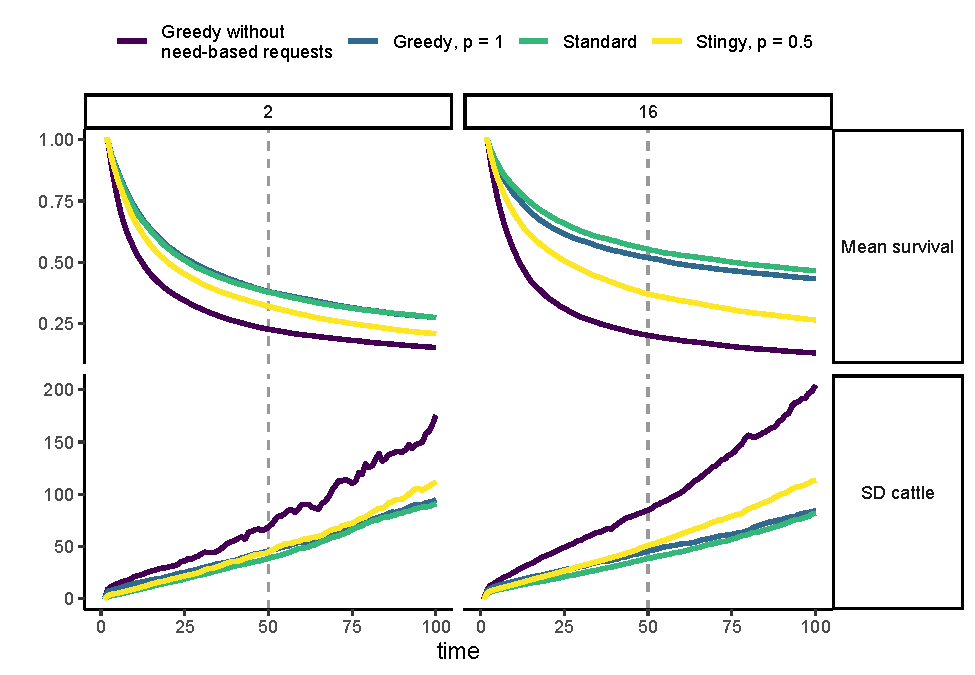
\includegraphics{needBasedSharing-paper_files/figure-latex/abmplot0-1.pdf}
\caption{\label{fig:abmplot0}Mean survival (top) and standard variation in herd sizes (bottom) over time. Left: group size = 2. Right: group size = 16. Colors represent models. Standard: The Aktipis et al.~(2011) ABM. Greedy: non-survival requests made in addition to need-based requests. Greedy without need-based requests: only greedy {[}non-survival based{]} requests are made (no need-based requests). Stingy: Need-based requests are refused with a probability of 0.5. The dashed line at t=50 shows where we calculated the survival advantage (or disadvantage) of partnerships.}
\end{figure}

We then re-ran this simulation across different partnership sizes (\(N\)) and \(p_G\) and \(p_S\) values. When we increased \(N\) for mutually cooperative partnerships (\(p_S=0\) and \(p_S=0\)), we saw higher survival outcomes. Further, and similar to the \(N=2\) results in Figure \ref{fig:abmplot0}, we saw that increasingly frequent greedy requests (\(p_G \rightarrow 1\) while \(p_S=0\)) had little-to-no impact on survival outcomes relative to the mutually cooperative outcomes. Hence, holding \(p_S\) to zero, increasing \(N\) substantially increased survival among all \(p_G \in [0,1]\). See Figure \ref{fig:abmplot1}. In contrast, increasing \(p_S\) from 0 to 1 reliably and substantially decreased survival across \(N\) values. Further, although survival when \(p_S=0\) increased as \(N\) increased, above moderate levels of stinginess, as partnership size increased from \(N=2\) to \(N=16\), survival outcomes were quicker to asymptote to \(\sim 25\%\) of agents surviving to \(t=50\). In other words, stingy defection becomes increasingly costly at a larger \(N\), because the difference in survival between \(p_S=0\) and \(p_S=1\) is positively associated with \(N\). See Figure \ref{fig:abmplot1}.

\begin{figure}
\centering
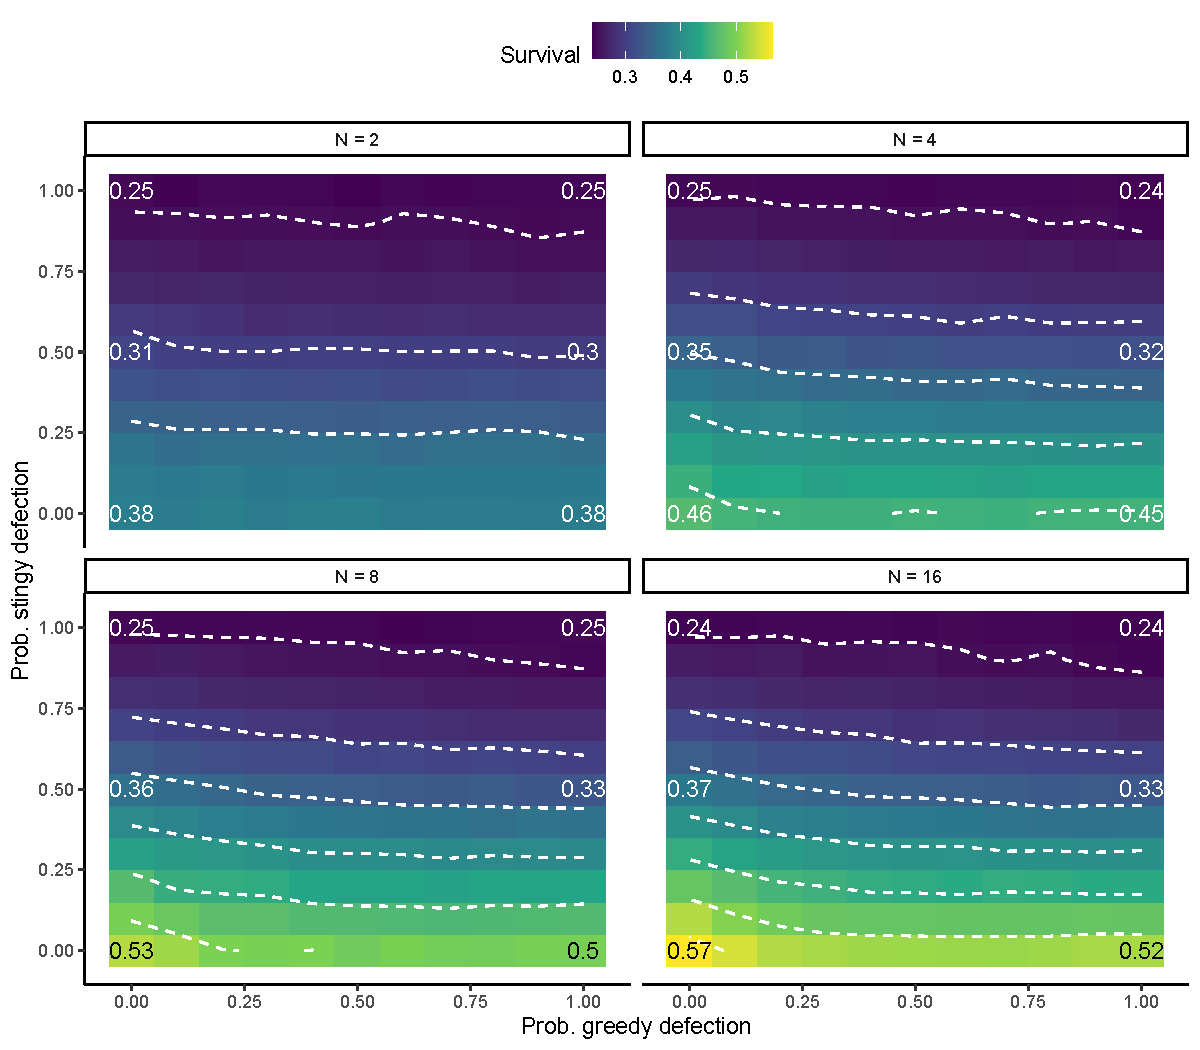
\includegraphics{needBasedSharing-paper_files/figure-latex/abmplot1-1.pdf}
\caption{\label{fig:abmplot1}Average survival outcomes after 50 time steps (color) across 100,000 simulation runs for each configuration of partnership sizes (N, shown here by facets), probability of stingy defection (y-axis), and probability of greedy defection (x-axis).}
\end{figure}

Taken together, these ABM results identify a critical caveat about need-based sharing: An interdependent need-based sharing institution like osotua is generally robust to greedy defection, but stingy defection always undermines its long-term sustainability. Further, because need-based sharing improves survival in increasingly large partnerships (even when greedy defectors are present), the relative importance of generosity, compared to detecting and preventing greedy requests, should be higher among larger need-based sharing partnerships. Put differently, stinginess becomes more costly as need-based sharing institutions scale to larger, more interconnected groups.

With a paradigmatic need-based sharing institution such as osotua, we can only resolve the typical size of a partnership and the extent to which Maasai tolerate non-survival requests with empirical data. To what extent will osotua partners respond to survival need-based vs.~non-survival requests with generosity? Are osotua partnerships restricted to dyads, or are they community-based, where we would expect greedy defection to be more likely to be tolerated?

\section{The experimental vignette: Testing the effect of need in Maasai osotua}\label{experiment}

In our empirical study, we conducted an experimental vignette with Kisongo Maasai pastoralists in Monduli Juu highlands of northern Tanzania (N = 218, 41.3\% female). We asked how each participant would respond to a request for assistance from a person with whom they had osotua. Prior to the vignette, each participant was given a structured survey that included measures of household food insecurity and social network data. The vignette and survey were administered by ADL with a Maasai translator or by one of two Maasai research assistants. All participants were paid 10,000 TZS (about \$4.35) for their participation, and all protocols and survey materials were approved by Washington State University IRB and Tanzanian Commission for Science and Technology (COSTECH) prior to data collection.

The experimental vignette described a hypothetical Maasai person with whom the participant had osotua, who has requested cattle to help him during a difficult time. The participant in this scenario was told that s/he had twenty cows at the time.\footnote{A fixed number of cattle was included in the vignette to keep the allocation numbers comparable between participants. Twenty cattle was specifically chosen because this was deemed a realistic number based on observation data collected by ADL during fieldwork. Herds in this region are often disaggregated across households, families, and friends, and frequent trading, selling, and buying means that herd sizes are relatively fluid from year to year. Basically, the hypothetical scenario outlined to participants was designed to be as realistic as possible to as many participants as possible.} Participants were randomly assigned to a condition in which this request was either based on \emph{survival need} (what models would call a genuine need-based request), because it involved resource scarcity after a drought, or \emph{non-survival need} (a greedy request), because it involved someone accumulating cattle to pay bridewealth for a second wife (N = 116 in the drought condition, N = 102 in the bridewealth condition).\footnote{We specifically used \emph{bridewealth for a second wife} in the non-survival need condition because although key informants stated that a first wife was important for having a family with children, more than one wife, while acceptable, is far less common.} We refer to this manipulated variable as the presence/absence of \emph{need}, where ``need'' refers to a condition that would cause relatively low chances of continued survival.

Consistent with the rules of a Dictator game, in which participants are given a resource allocation and must decide how much of it to share, participants were asked how many of their cows they would share with the person in the vignette requesting help. This number of cows shared, between 0 and 20, was the outcome measure of interest, which we refer to as \emph{shared}. The structured survey included household food insecurity scores (Blumberg et al. 1999), which we refer to as \emph{insecure}. Because the rules of need-based sharing include a caveat where individuals must share if they are able to, our confirmatory models controlled for food insecurity scores, a proxy for reduced sharing ability. Hence, the linear regression model used in our confirmatory analysis was

\[
\text{share} = \alpha + \beta_1 \times \text{need} + \beta_2 \times \text{insecure}
\]

where we predicted that \(\beta_1 > 0\), \(p < 0.05\). We used social network data for exploratory analyses. Social network data consisted of egocentric networks, created after asking participants to list the people with whom they had the most osotua. As we will discuss further below, we collected social network data by asking participants with whom they had the most osotua, which allowed us to count the number of people mentioned per participant. Participants frequently volunteered more information about osotua during this part of the survey, and we collected these statements for additional context.

Preregistration materials can be found at \href{https://osf.io/ndfxc}{osf.io/ndfxc}, and the anonymized experimental and structured survey data can be found at \href{https://github.com/alightner/needBasedSharing-study}{github.com/alightner/needBasedSharing-study}.

\subsection{Results of the experiment}

We found that survival need increased the amount shared (\(\beta\) = 0.42, \(p\) = 0.044, \(SE\) = 0.21), controlling for household food insecurity (Blumberg et al. 1999), a proxy for reduced sharing ability (\(\beta\) = 0.014, \(p\) = 0.96, \(SE\) = 0.3). Simplifying our model by not controlling for food insecurity -- which deviates from our preregistered analysis plan -- did not alter the positive causal effect of survival need on amount shared (\(\beta\) = 0.42, \(p\) = 0.043, \(SE\) = 0.21).

Nevertheless, most participants were willing to share small numbers of cattle even when survival need was absent. Despite amounts shared being slightly higher for need-based requests, both conditions elicited similar levels of generosity (drought: mean = 2.8, median = 3, sd = 1.3; bridewealth: mean = 2.4, median = 2, sd = 1.7; Mann-Whitney U = 7507, \(p\) = \ensuremath{1.8\times 10^{-4}}), and out of the 218 participants in this experiment, only 1 participant refused to share anything. See Figure \ref{fig:amtshareplot}.

\begin{figure}
\centering
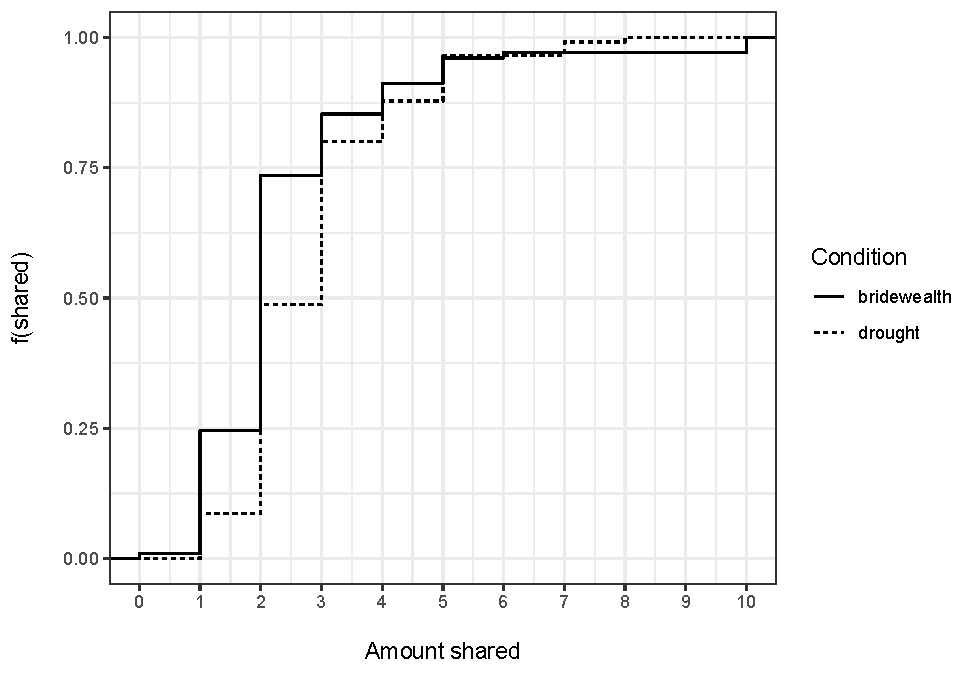
\includegraphics{needBasedSharing-paper_files/figure-latex/amtshareplot-1.pdf}
\caption{\label{fig:amtshareplot}Empirical cumulative distribution of the reported amounts of cattle that participants were willing to share, by experimental condition. Amounts were out of an initial resource holding of twenty head of cattle.}
\end{figure}

In our exploratory analysis, we assessed the scale of osotua partnerships using qualitative and observational data, interview data from key informants, and social network data from each participant. Qualitative and observational data suggested that osotua is a large-scale, community-level institution: when participants were asked with whom they had osotua, a common response was ``everyone.'' This was not surprising after our initial key informant interviews, where people referred to osotua as a perspective, a personality characteristic akin to generosity and kindness, and/or ``comfort.'' According to some informants, examples of ``comfort'' included helpful acts during times of distress, such as offering a Maasai stranger food and shelter when s/he is far from home, or helping a warrior calm his nerves before his circumcision ceremony. As a first pass, these ethnographic data suggest that osotua is indeed a broad institution (i.e., many connected to many) for Kisongo Maasai.

The participants' views of osotua as a community-level phenomenon made collecting social network data about osotua partnerships challenging. We addressed this challenge by asking participants, ``with whom do you have \emph{the most} osotua?'' Consistent with our initial observations, many individuals had many relatively close osotua partners, even after restricting their responses to their closest and most salient partners (Figure \ref{fig:degosotuaplot}).\footnote{Many of the names given during the social network data collection phase had included mentions that were not included in our sample. These represent the boundaries of our social network, and this is a primary reason why we focus here on the number of ties per participant rather than a complete sociocentric network.}

\begin{figure}
\centering
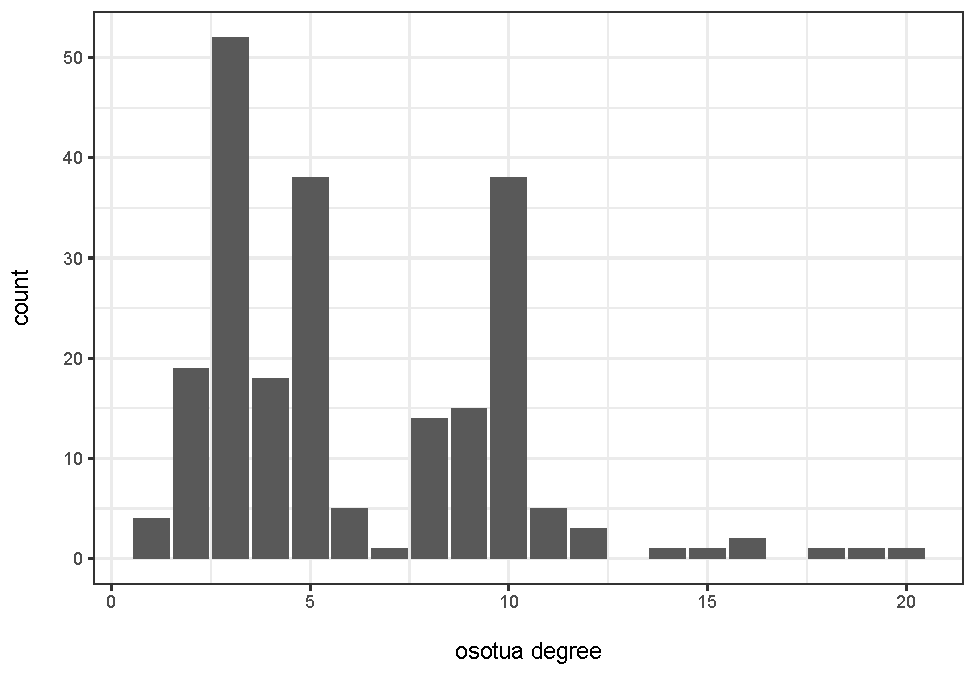
\includegraphics{needBasedSharing-paper_files/figure-latex/degosotuaplot-1.pdf}
\caption{\label{fig:degosotuaplot}Counts of the number of mentioned names that each participant gave when asked with whom he or she had the most osotua.}
\end{figure}

Our main results revealed a positive effect of need on sharing, and as we and others have shown, need-based sharing in osotua \emph{can} reduce potential risks to survival. To evaluate whether or not this might actually be the case, we analyzed the impact of having more vs.~fewer close osotua partners on household food insecurity, finding a curvilinear association between number of osotua partners and food insecurity scores. Consistent with risk pooling accounts of need-based sharing, food insecurity was negatively associated with the number of close osotua ties among individuals with fewer ties (number of osotua partners: \(\beta=\) -0.056, \(p=\) \ensuremath{3.2\times 10^{-4}}, \(SE\) = 0.015; number of osotua partners squared: \(\beta=\) 0.0021, \(p=\) 0.0088, \(SE\) = \ensuremath{8.1\times 10^{-4}}; see Figure \ref{fig:osotuainsecure}).

\begin{figure}
\centering
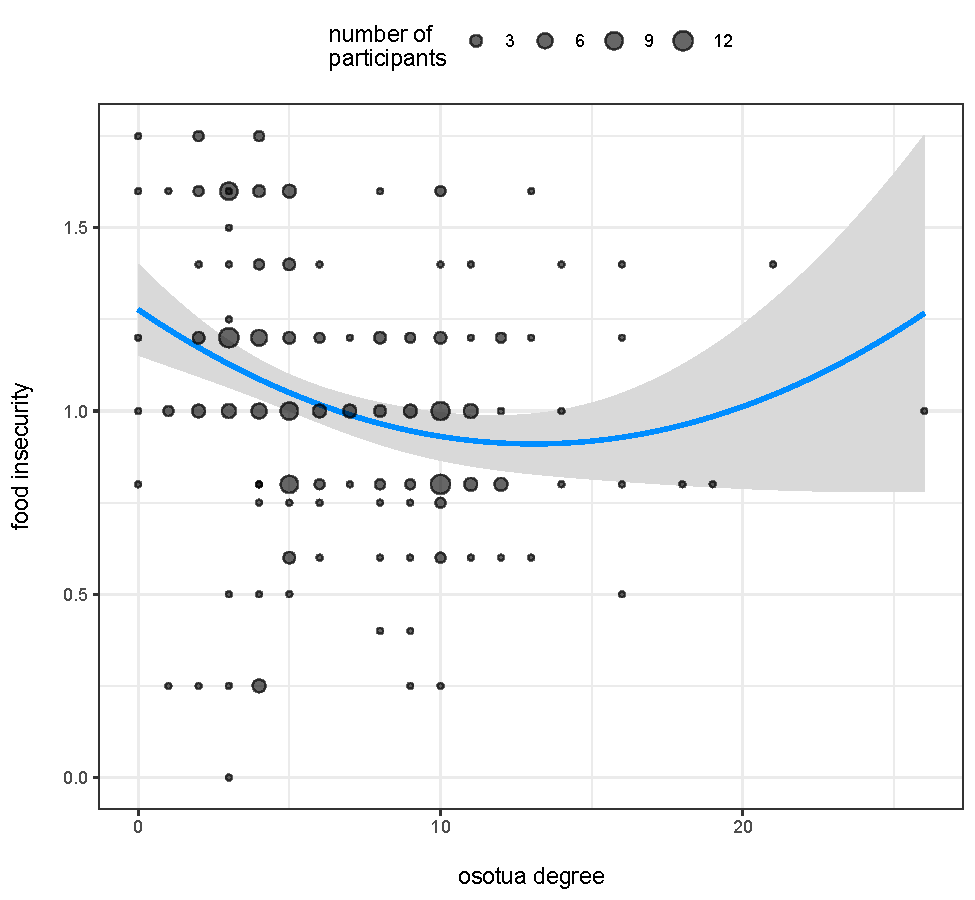
\includegraphics{needBasedSharing-paper_files/figure-latex/osotuainsecure-1.pdf}
\caption{\label{fig:osotuainsecure}Regression model of household food insecurity scores as a function of number of osotua partners, based on a social network of close osotua partnerships. Larger points indicate a greater number of participants with a given osotua degree and level of food insecurity.}
\end{figure}

\section{Discussion}\label{discussion}

In this study we investigated Maasai osotua, a paradigmatic example of a need-based sharing institution that reduces individuals' risk, improving long-term survival prospects (Aktipis et al. 2016; Campenni, Cronk, and Aktipis 2017; Cronk and Aktipis 2021). A challenge for need-based sharing institutions, which many other cooperative institutions also face, is that societies must somehow motivate individuals to cooperate while reducing temptations to defect. Need-based sharing has two potential sources of defection --- refusing to help someone when they ask for help (the stingy strategy) and asking for help when risks to survival are not present (the greedy strategy) --- and existing models have not considered each separately. Yet, a vulnerability of need-based sharing is the potential ambiguity between genuinely need-based vs.~greedy requests: Individuals might colloquially justify their claims about ``genuine need'' in ways that do not conform to its standard uses in formal and evolutionary models, which tend to narrowly focus on risks to continued survival.

In an agent-based model (ABM), we extended the ABM of Aktipis, Cronk, and Aguiar (2011), a dyadic model without defection, to both expand the size of need-based partnerships (e.g., Hao et al. 2015; Kayser and Armbruster 2016; Campenni, Cronk, and Aktipis 2021) and to distinguish greedy defection from stingy defection. Distinguishing greedy from stingy defection suggests that sharing, and not just sharing based on need, may underlie the long-term survival benefits that need-based sharing institutions offer: need-based sharing is resilient against greedy defection as long as need-based requests still occur, but is not resilient against stingy defection (Figure \ref{fig:abmplot0}). Further, increasing the size of need-based sharing partnerships also increases the benefits of risk pooling, and as they increase in size, these partnerships remain resilient to greedy defection. On the other hand, stingy defection is increasingly costly as partnership sizes increase (Figure \ref{fig:abmplot1}). We therefore identify a subtlety in the boundary conditions of need-based sharing institutions: Assuming interdependence, greediness is easily tolerated but stinginess is not -- and it becomes increasingly costly as partnerships increase in size.

We can consider the behavioral implications of this asymmetry between greedy vs.~stingy behavior using error management theory (Haselton et al. 2009; McKay and Efferson 2010) and the multiplicative growth of assets---both cattle herds and networks of cooperators (Dyson-Hudson and Dyson-Hudson 1980; Lesorogol 2009; Bollig 2010; Price and Jones 2020). Consider the decision task for need-based sharing partners in an institution like osotua. Each agent takes on a scenario-specific role at each time step: a potential \emph{recipient} who can send a signal for aid, and a potential \emph{donor} who receives that signal. At each time step, the recipient sends a potentially ambiguous signal, which was either generated by a state of need or a state of ``greed.'' Under such ambiguity, the expected cost of stinginess toward needy requests (\(p_S >0\) and \(p_G=0\) in the ABM) always outweighs the expected cost of sharing with greedy requests (\(p_G>0\) and \(p_S=0\) in the ABM; see Figure \ref{fig:abmplot1}), because the cost of rejecting a genuine request is high. To understand this cost, first consider the cost to the herd of rejecting a genuine request. Because of the multiplicative nature of herd growth, rare shocks are amplified, meaning each individual's resource level is constantly trending toward zero (Peters and Gell-Mann 2016; Price and Jones 2020). Interdependence reduces the risk of hitting zero (Kelley and Thibaut 1978; Roberts 2005; Balliet, Tybur, and Van Lange 2017; Aktipis et al. 2018; Gerpott et al. 2018; Price and Jones 2020; Campenni, Cronk, and Aktipis 2021). Second, individuals have to stay alive to help one another in future instances of need, but because of the interdependence fostered by need-based institutions, shocks again have multiplicative effects. Assuming greedy individuals are willing to help in future instances of need (i.e., when \(p_S \approx 0\)), then when greedy defectors supplement their need-based requests with non-survival ones, they improve their own chances of surviving long enough to help each other in future instances of need. Future research could investigate the similarities and differences between the resource dynamics in need-based sharing (with or without non-survival requests) and group-level pooling strategies, the latter being an effective means of reducing variance around annual growth rates (and potential losses) (Price and Jones 2020; Peters and Adamou 2022).

Results from our empirical field study among Tanzanian Kisongo Maasai pastoralists were consistent with these insights. Supporting a need-based sharing account of osotua, we found that participants were willing to share more cattle when an osotua request was based on survival need (feeding one's family after a drought) rather than non-survival need (obtaining bridewealth for a second wife). We also found that, for most people, that individuals who were more involved in osotua partnerships had lower household food insecurity scores -- with the exception of a few individuals with very large numbers of osotua partners, reflected in the curvilinear relationship (Figures \ref{fig:amtshareplot} and \ref{fig:osotuainsecure}). This exception might reflect a high demand among individuals with many osotua partnerships, which we will discuss further below. Importantly, though, participants frequently complied with non-survival need-based, or ``greedy,'' requests. Our interview data also suggested that osotua is an important and broad, community-level institution, and generosity in osotua was frequently described as something that should be applied to other Maasai people across many facets of life. Informants gave examples of how and when osotua can occur beyond formal cattle sharing partnerships -- like about how it can even include behaviors such as hospitality toward a traveling stranger. During social network data collection, even when we restricted participants' responses to the most salient and important osotua ties, participants reported widespread community involvement in osotua: many participants have many close ties (Figure \ref{fig:degosotuaplot}).

Taken together, our models and experimental vignette findings suggest a broad, testable framework that expands on the work of Aktipis, Cronk, and others. While our results support the claim that osotua is a need-based sharing institution that beneficially pools risk (Aktipis, Cronk, and Aguiar 2011; Aktipis et al. 2016, 2018; Campenni, Cronk, and Aktipis 2021), the asymmetry between costs of greed vs.~stinginess shows that sharing is generally favored, even when greedy requests might be prevalent. In future research we would expect that in institutions with need-based sharing and interdependence, people err on the side of sharing, rather than rejecting, a potentially frivolous request. We would also expect this to tendency to increase as environments become harsher and more volatile, and as partnerships increase in size and levels of perceived interdependence (Balliet, Tybur, and Van Lange 2017; Gerpott et al. 2018). Specifically, we would predict that need-based sharing among many densely connected individuals is more tolerant of non-survival requests (as we observed in our field study with Tanzanian Maasai pastoralists), compared to rigid, dyadic partnerships (e.g., in a sparse and/or controlled social network) (Aktipis 2004; Baumard, André, and Sperber 2013; Pisor and Gurven 2018). Conversely, while we would expect that generosity would be more central to need-based sharing institutions than restraint from making non-survival requests, we would expect restraint to become more important when greedy requests become excessively frequent, and when environments and subsistence strategies become more stable.

Our results reframe ongoing conversations about the nature of human sociality, specifically with respect to how ``need'' works on the ground, how osotua works, and how need-based sharing is or is not distinct from delayed reciprocity. First, evolutionary models tend to characterize ``need'' in terms of continued survival prospects, and as we show, some culturally acceptable ways of justifying need are formally equivalent to the greedy strategy -- even in osotua, the touchstone example of need-based sharing. Future research could apply a similar approach to other evolutionary theories by investigating the extent to which theoretical constructs in our formal models actually map onto folk constructs ``on the ground'' in a given cultural context (e.g., Stibbard-Hawkes, Smith, and Apicella 2022).

Second, a compelling avenue for future research would be to investigate how need-based sharing and delayed reciprocity are related but differentially expressed as a consequence of different social and environmental contexts. Our findings resemble key characteristics of delayed reciprocity, where future returns are somehow expected, but strict book-keeping is not (Wiessner 2002). Indeed, during fieldwork, multiple informants told ADL a common Kisongo Maasai saying about osotua: \emph{engiteng osotua elo eshukunyie} (translated from Maa: ``whatever cow I give in osotua will someday come back'' -- if not from one osotua partner, from another). Higher vs.~lower levels of interdependence might account for how people deem non-need-based requests as unacceptable vs.~acceptable, and community-level need-based sharing practices that we observed in this study also seemed to bear key similarities to the demand sharing practices, for example, that have been documented among some forager groups (Jones 1984; Blurton Jones 1987; Peterson 1993). In such cases, requests are frequent and not necessarily based on need, but an expectation of generosity compels people to share small amounts. In the osotua case, this results in generalized reciprocity (Rankin and Taborsky 2009) -- widespread sharing among people with whom one has osotua, based on having experienced sharing before, not tit for tat. In future work, a more general theory of sharing as risk reduction could unify these apparently separate modes of cooperation (Winterhalder 1996; Bird and Bird 1997; Iyer 2016).

Third, our findings suggest that for Kisongo Maasai, osotua is less akin to a formal partnership and more akin to a broad, community-level need-based sharing ``ethos'' in which non-survival requests are acceptable. It is nevertheless conceivable that need-based sharing in other cultural contexts \emph{is less} forgiving of non-survival requests. Cronk (2007), for example, found that among the Mukugodo Maasai, non-need-based requests among osotua partners were ``unthinkable'' (p.~353). Our findings do not contradict Cronk's, but complement them: Mukogodo Maasai of Kenya are geographically quite distant from the Kisongo Maasai of northern Tanzania, and their histories are very different (Spear and Waller 1993; Cronk 2004). Based on the theoretical framework that we have laid out here, osotua for Mukogodo Maasai might reflect a history of demand sharing as former foragers (rather than account-keeping; see also Iyer (2016)), possibly with a social structure with far less redundancy among sharing network ties than those observed among Kisongo Maasai.

\subsection{Limitations}

Our study has a few limitations. The ABM, for simplicity, assumes that increasingly large partnerships are completely connected communities. Network structure can play an influential role in need-based sharing (Hao et al. 2015; Kayser and Armbruster 2016), but we currently lack the empirical data to create a clear and detailed picture of how osotua networks are structured at the society level. Additionally, our ABM does not determine if the strategies we investigate can evolve over the course of multiple generations.

Our field evidence that individuals with more close osotua partners had lower household food insecurity was not a preregistered hypothesis, but a post hoc exploratory finding, and therefore has a higher risk of being spurious. Additionally, whereas we interpret the result as more support from osotua translating to lower-risk livelihoods, it might instead suggest that fewer resources translates to lower partner value, leading to fewer osotua partners. However, this interpretation would conflict with the observation that osotua partnerships often originate in childhood, and can even be passed down to one's children (Spencer 1965; Cronk 2007) (although wealth is also transmitted between generations among many pastoralist groups, so more direct research would be needed to address this; see Borgerhoff Mulder et al. (2010)).

Further, we did not systematically investigate how people subjectively approved or disapproved of the requests in the experimental vignette. We thus inferred participants' approval based on their sharing behavior, although our key informants suggested that the bridewealth requests were neither taboo nor inappropriate. We also did not test the extent to which people prioritized sharing unconditionally, without expectation of future help, or how important people thought it was to be generous rather than stingy in the osotua interaction we described in the vignette. Our key informant interviews and observational evidence did suggest that generosity was extremely important, but because costly stinginess was so central to our theoretical results, future research should directly test our inferences that rules against greedy defection should be less stringent than rules against stingy defection.

\section{Conclusion}

Evolutionary theories of cooperation suggest that need-based sharing is a critical part of human cultures everywhere (Hruschka 2010; Cronk et al. 2019). These theories suggest that need-based sharing practices follow two simple rules: help others when asked, and only ask for help when genuine need arises. Formally, genuine need is typically defined in terms of long-term survival risks, but cross-culturally and colloquially, its criteria might vary. In an experimental vignette, we investigated how and why Tanzanian Kisongo Maasai pastoralists respond to requests in osotua, a paradigmatic example of need-based sharing, that were either based on survival need (needing subsistence after a drought) or non-survival need (needing bridewealth to acquire a second wife). We found that requests based on survival need were weakly associated with more cattle sharing than requests based on non-survival need. Sharing was widespread across both conditions, however, and participants were almost always willing to share small amounts. In an ABM, we showed why this might be the case: interdependent need-based sharing partnerships can easily tolerate greediness, but they do not tolerate stinginess -- especially in large, interconnected partnerships like osotua among the Kisongo Maasai. In need-based sharing, stinginess is far worse than greed.

\section*{Acknowledgements}

We especially thank the Maasai people who participated in this study. We also thank Musa Kamaika, Kotoke Ngilepoi, and an anonymous Maasai research assistant for invaluable aid during the field study. We acknowledge funding from a National Science Foundation Doctoral Dissertation Improvement Grant (award number 1918523), and ADL acknowledges funding from the Aarhus University Research Foundation.

\section*{Conflicts of Interest}

None.

\section*{References}

\hypertarget{refs}{}
\begin{CSLReferences}{1}{0}
\leavevmode\hypertarget{ref-aktipisathenaPrinciplesCooperationSystems2015}{}%
Aktipis, Athena. 2015. {``Principles of Cooperation Across Systems: From Human Sharing to Multicellularity and Cancer.''} \emph{Evolutionary Applications} 9(1):17--36. doi: \href{https://doi.org/10.1111/eva.12303}{10.1111/eva.12303}.

\leavevmode\hypertarget{ref-aktipisUnderstandingCooperationFitness2018}{}%
Aktipis, Athena, Lee Cronk, Joe Alcock, Jessica D. Ayers, Cristina Baciu, Daniel Balliet, Amy M. Boddy, Oliver Scott Curry, Jaimie Arona Krems, Andrés Muñoz, Daniel Sullivan, Daniel Sznycer, Gerald S. Wilkinson, and Pamela Winfrey. 2018. {``Understanding Cooperation Through Fitness Interdependence.''} \emph{Nature Human Behaviour} 2(7):429--31. doi: \href{https://doi.org/10.1038/s41562-018-0378-4}{10.1038/s41562-018-0378-4}.

\leavevmode\hypertarget{ref-aktipisCooperationUncertainWorld2016}{}%
Aktipis, Athena, Rolando de Aguiar, Anna Flaherty, Padmini Iyer, Dennis Sonkoi, and Lee Cronk. 2016. {``Cooperation in an {Uncertain World}: {For} the {Maasai} of {East Africa}, {Need}-{Based Transfers Outperform Account}-{Keeping} in {Volatile Environments}.''} \emph{Human Ecology} 44:353--64. doi: \href{https://doi.org/10.1007/s10745-016-9823-z}{10.1007/s10745-016-9823-z}.

\leavevmode\hypertarget{ref-aktipis2004know}{}%
Aktipis, C. Athena. 2004. {``Know When to Walk Away: Contingent Movement and the Evolution of Cooperation.''} \emph{Journal of Theoretical Biology} 231(2):249--60.

\leavevmode\hypertarget{ref-aktipisRiskPoolingHerdSurvival2011}{}%
Aktipis, C. Athena, Lee Cronk, and Rolando de Aguiar. 2011. {``Risk-{Pooling} and {Herd Survival}: {An Agent}-{Based Model} of a {Maasai Gift}-{Giving System}.''} \emph{Human Ecology} 39(2):131--40. doi: \href{https://doi.org/10.1007/s10745-010-9364-9}{10.1007/s10745-010-9364-9}.

\leavevmode\hypertarget{ref-ballietFunctionalInterdependenceTheory2017}{}%
Balliet, Daniel, Joshua M. Tybur, and Paul A. M. Van Lange. 2017. {``Functional {Interdependence Theory}: {An Evolutionary Account} of {Social Situations}.''} \emph{Personality and Social Psychology Review} 21(4):361--88. doi: \href{https://doi.org/10.1177/1088868316657965}{10.1177/1088868316657965}.

\leavevmode\hypertarget{ref-baumard2013mutualistic}{}%
Baumard, Nicolas, Jean-Baptiste André, and Dan Sperber. 2013. {``A Mutualistic Approach to Morality: The Evolution of Fairness by Partner Choice.''} \emph{Behavioral and Brain Sciences} 36(1):59--78.

\leavevmode\hypertarget{ref-bird1997delayed}{}%
Bird, Rebecca L. Bliege, and Douglas W. Bird. 1997. {``Delayed Reciprocity and Tolerated Theft: The Behavioral Ecology of Food-Sharing Strategies.''} \emph{Current Anthropology} 38(1):49--78.

\leavevmode\hypertarget{ref-blumbergEffectivenessShortForm1999}{}%
Blumberg, S. J., K. Bialostosky, W. L. Hamilton, and R. R. Briefel. 1999. {``The Effectiveness of a Short Form of the {Household Food Security Scale}.''} \emph{American Journal of Public Health} 89(8):1231--34.

\leavevmode\hypertarget{ref-blurton1987tolerated}{}%
Blurton Jones, Nicholas G. 1987. {``Tolerated Theft, Suggestions about the Ecology and Evolution of Sharing, Hoarding and Scrounging.''} \emph{Social Science Information} 26(1):31--54.

\leavevmode\hypertarget{ref-bolligRiskManagementHazardous2010}{}%
Bollig, Michael. 2010. \emph{Risk Management in a Hazardous Environment: {A} Comparative Study of Two Pastoral Societies}. Vol. 2. {Springer Science \& Business Media}.

\leavevmode\hypertarget{ref-borgerhoffmulderPastoralismWealthInequality2010}{}%
Borgerhoff Mulder, Monique, Ila Fazzio, William Irons, Richard L. McElreath, Samuel Bowles, Adrian Bell, Tom Hertz, and Leela Hazzah. 2010. {``Pastoralism and {Wealth Inequality}: {Revisiting} an {Old Question}.''} \emph{Current Anthropology} 51(1):35--48. doi: \href{https://doi.org/10.1086/648561}{10.1086/648561}.

\leavevmode\hypertarget{ref-campenniCorrelatedDisastersNeedbased2017}{}%
Campenni, Marco, Lee Cronk, and Athena Aktipis. 2017. {``Correlated Disasters and Need-Based Transfers: {The} Limits of Risk Pooling Systems in Simulated Ecologies.''} doi: \href{https://doi.org/10.1101/230607}{10.1101/230607}.

\leavevmode\hypertarget{ref-campenni2021need}{}%
Campenni, Marco, Lee Cronk, and Athena Aktipis. 2021. {``Need-Based Transfers Enhance Resilience to Shocks: An Agent-Based Model of a Maasai Risk-Pooling System.''} \emph{Human Ecology} 1--14.

\leavevmode\hypertarget{ref-claessensNeedbasedTransferSystems2021}{}%
Claessens, Scott, Jessica D. Ayers, Lee Cronk, and Athena Aktipis. 2021. {``Need-Based Transfer Systems Are More Vulnerable to Cheating When Resources Are Hidden.''} \emph{Evolution and Human Behavior} 42(2):104--12. doi: \href{https://doi.org/10.1016/j.evolhumbehav.2020.08.004}{10.1016/j.evolhumbehav.2020.08.004}.

\leavevmode\hypertarget{ref-cronkUnfamiliarSocialNorm2008}{}%
Cronk, L., and H. Wasielewski. 2008. {``An Unfamiliar Social Norm Rapidly Produces Framing Effects in an Economic Game.''} \emph{Journal of Evolutionary Psychology} 6(4):283--308. doi: \href{https://doi.org/10.1556/JEP.6.2008.4.3}{10.1556/JEP.6.2008.4.3}.

\leavevmode\hypertarget{ref-cronkMukogodoMaasaiEthnicity2004}{}%
Cronk, Lee. 2004. \emph{From {Mukogodo} to {Maasai}: Ethnicity and Cultural Change in {Kenya}}. {Boulder, Colo}: {Westview Press}.

\leavevmode\hypertarget{ref-cronkInfluenceCulturalFraming2007}{}%
Cronk, Lee. 2007. {``The Influence of Cultural Framing on Play in the Trust Game: A {Maasai} Example.''} \emph{Evolution and Human Behavior} 28(5):352--58. doi: \href{https://doi.org/10.1016/j.evolhumbehav.2007.05.006}{10.1016/j.evolhumbehav.2007.05.006}.

\leavevmode\hypertarget{ref-cronk2021design}{}%
Cronk, Lee, and Athena Aktipis. 2021. {``Design Principles for Risk-Pooling Systems.''} \emph{Nature Human Behaviour} 5(7):825--33.

\leavevmode\hypertarget{ref-cronkManagingRiskCooperationinpress}{}%
Cronk, Lee, Colette Berbesque, Thomas Conte, Matthew Gervais, Iyer Padmini, Brighid McCarthy, Dennis Sonkoi, Cathryn Townsend, and Athena Aktipis. 2019. {``Managing Risk Through Cooperation: {Need}-Based Transfers and Risk Pooling Among the Societies of the {Human Generosity Project}.''} in \emph{Global perspectives on long term community resource management}. {Springer}.

\leavevmode\hypertarget{ref-cronkSolidarityTypeWorldNeedBased2021}{}%
Cronk, Lee, Diego Guevara Beltrán, Denise Laya Mercado, and Athena Aktipis. 2021. {``{`{A Solidarity}-{Type World}'}: {Need}-{Based Helping} Among {Ranchers} in the {Southwestern United States}.''} \emph{Human Nature}. doi: \href{https://doi.org/10.1007/s12110-021-09406-8}{10.1007/s12110-021-09406-8}.

\leavevmode\hypertarget{ref-dyson-hudsonNomadicPastoralism1980}{}%
Dyson-Hudson, Rada, and Neville Dyson-Hudson. 1980. {``Nomadic Pastoralism.''} \emph{Annual Review of Anthropology} 9(1):15--61.

\leavevmode\hypertarget{ref-eshelPartnership2001}{}%
Eshel, ILAN, and AVNER Shaked. 2001. {``Partnership.''} \emph{Journal of Theoretical Biology} 208(4):457--74. doi: \href{https://doi.org/10.1006/jtbi.2000.2232}{10.1006/jtbi.2000.2232}.

\leavevmode\hypertarget{ref-garayCooperationDefencePredator2009}{}%
Garay, József. 2009. {``Cooperation in Defence Against a Predator.''} \emph{Journal of Theoretical Biology} 257(1):45--51. doi: \href{https://doi.org/10.1016/j.jtbi.2008.11.010}{10.1016/j.jtbi.2008.11.010}.

\leavevmode\hypertarget{ref-gerpottHowPeopleThink2018}{}%
Gerpott, Fabiola H., Daniel Balliet, Simon Columbus, Catherine Molho, and Reinout E. de Vries. 2018. {``How Do People Think about Interdependence? {A} Multidimensional Model of Subjective Outcome Interdependence.''} \emph{Journal of Personality and Social Psychology} 115(4):716--42. doi: \href{https://doi.org/10.1037/pspp0000166}{10.1037/pspp0000166}.

\leavevmode\hypertarget{ref-haoNeedbasedTransfersNetwork2015}{}%
Hao, Yan, Dieter Armbruster, Lee Cronk, and C. Athena Aktipis. 2015. {``Need-Based Transfers on a Network: A Model of Risk-Pooling in Ecologically Volatile Environments.''} \emph{Evolution and Human Behavior} 36(4):265--73. doi: \href{https://doi.org/10.1016/j.evolhumbehav.2014.12.003}{10.1016/j.evolhumbehav.2014.12.003}.

\leavevmode\hypertarget{ref-haseltonAdaptiveRationalityEvolutionary2009a}{}%
Haselton, Martie, Gregory Bryant, Andreas Wilke, David Frederick, Andrew Galperin, Willem Frankenhuis, and Tyler Moore. 2009. {``Adaptive Rationality: {An} Evolutionary Perspective on Cognitive Bias.''} \emph{Psychology Faculty Articles and Research}.

\leavevmode\hypertarget{ref-hollisNoteMasaiSystem1910}{}%
Hollis, Alfred C. 1910. {``A {Note} on the {Masai System} of {Relationship} and {Other Matters Connected Therewith}.''} \emph{The Journal of the Royal Anthropological Institute of Great Britain and Ireland} 40:473--82.

\leavevmode\hypertarget{ref-hruschkaFriendshipDevelopmentEcology2010}{}%
Hruschka, Daniel J. 2010. \emph{Friendship: {Development}, Ecology, and Evolution of a Relationship}. Vol. 5. {Univ of California Press}.

\leavevmode\hypertarget{ref-iyer2016risk}{}%
Iyer, K. Padmini. 2016. {``Risk Management Through Social Networks Among Male and Female Pastoralists in Karamoja, Uganda.''} PhD thesis, Rutgers University-Graduate School-New Brunswick.

\leavevmode\hypertarget{ref-jacobsTraditionalPoliticalOrganization1965}{}%
Jacobs, Alan. 1965. {``The Traditional Political Organization of the Pastoral {Maasai}.''} Ph.\{\{D\}\}. Dissertation, Anthropology, University of California - Los Angeles.

\leavevmode\hypertarget{ref-johnstoneContinuousSirPhilip1992}{}%
Johnstone, Rufus A., and Alan Grafen. 1992. {``The Continuous {Sir Philip Sidney} Game: {A} Simple Model of Biological Signalling.''} \emph{Journal of Theoretical Biology} 156(2):215--34. doi: \href{https://doi.org/10.1016/S0022-5193(05)80674-5}{10.1016/S0022-5193(05)80674-5}.

\leavevmode\hypertarget{ref-jones1984selfish}{}%
Jones, NG Blurton. 1984. {``A Selfish Origin for Human Food Sharing: Tolerated Theft.''} \emph{Ethology and Sociobiology} 5(1):1--3.

\leavevmode\hypertarget{ref-kayserEconomicsNeedbasedTransfers2018}{}%
Kayser, Kirk. 2018. {``The Economics of Need-Based Transfers.''} \{\{PhD\}\} Dissertation, \{\{Applied Mathematics\}\}, Arizona State University.

\leavevmode\hypertarget{ref-kayserSocialOptimaNeedbased2016}{}%
Kayser, Kirk, and Dieter Armbruster. 2016. {``Social {Optima} of {Need}-Based {Transfers}.''}

\leavevmode\hypertarget{ref-kelleyInterpersonalRelationsTheory1978}{}%
Kelley, Harold H., and John W. Thibaut. 1978. \emph{Interpersonal Relations: A Theory of Interdependence}. {New York}: {Wiley}.

\leavevmode\hypertarget{ref-lee1979kung}{}%
Lee, Richard Borshay. 1979. \emph{The !kung San: Men, Women and Work in a Foraging Society}. Cambridge University Press.

\leavevmode\hypertarget{ref-lesorogolAssetBuildingCommunity2009}{}%
Lesorogol, Carolyn K. 2009. {``Asset Building Through Community Participation: Restocking Pastoralists Following Drought in Northern {Kenya}.''} \emph{Social Work in Public Health} 24(1-2):178--86. doi: \href{https://doi.org/10.1080/19371910802569740}{10.1080/19371910802569740}.

\leavevmode\hypertarget{ref-maynard-smithAnimalSignals2003}{}%
Maynard-Smith, John, and David Harper. 2003. \emph{Animal {Signals}}. 1 edition. {New York}: {Oxford University Press}.

\leavevmode\hypertarget{ref-mckay2010subtleties}{}%
McKay, Ryan, and Charles Efferson. 2010. {``The Subtleties of Error Management.''} \emph{Evolution and Human Behavior} 31(5):309--19.

\leavevmode\hypertarget{ref-mercierEnigmaReason2017}{}%
Mercier, Hugo, and Dan Sperber. 2017. \emph{The Enigma of Reason}. {Cambridge, Massachusetts}: {Harvard University Press}.

\leavevmode\hypertarget{ref-perlovTradingInfluenceSocial1987}{}%
Perlov, D. C. 1987. {``Trading for Influence: {The} Social and Cultural Economics of Livestock Marketing Among the Highland {Samburu} of {Northern Kenya}.''} Ph.\{\{D\}\}. Dissertation, Anthropology, University of California - Los Angeles.

\leavevmode\hypertarget{ref-petersEvaluatingGamblesUsing2016}{}%
Peters, O., and M. Gell-Mann. 2016. {``Evaluating Gambles Using Dynamics.''} \emph{Chaos: An Interdisciplinary Journal of Nonlinear Science} 26(2):023103. doi: \href{https://doi.org/10.1063/1.4940236}{10.1063/1.4940236}.

\leavevmode\hypertarget{ref-peters2022ergodicity}{}%
Peters, Ole, and Alexander Adamou. 2022. {``The Ergodicity Solution of the Cooperation Puzzle.''} \emph{Philosophical Transactions of the Royal Society A} 380(2227):20200425.

\leavevmode\hypertarget{ref-peterson1993demand}{}%
Peterson, Nicolas. 1993. {``Demand Sharing: Reciprocity and the Pressure for Generosity Among Foragers.''} \emph{American Anthropologist} 95(4):860--74.

\leavevmode\hypertarget{ref-pisor2018diversify}{}%
Pisor, Anne C., and Michael Gurven. 2018. {``When to Diversify, and with Whom? Choosing Partners Among Out-Group Strangers in Lowland Bolivia.''} \emph{Evolution and Human Behavior} 39(1):30--39.

\leavevmode\hypertarget{ref-priceFitnessmaximizersEmployPessimistic2020}{}%
Price, Michael Holton, and James Holland Jones. 2020. {``Fitness-Maximizers Employ Pessimistic Probability Weighting for Decisions Under Risk.''} \emph{Evolutionary Human Sciences} 2. doi: \href{https://doi.org/10.1017/ehs.2020.28}{10.1017/ehs.2020.28}.

\leavevmode\hypertarget{ref-rankin2009assortment}{}%
Rankin, Daniel J., and Michael Taborsky. 2009. {``Assortment and the Evolution of Generalized Reciprocity.''} \emph{Evolution: International Journal of Organic Evolution} 63(7):1913--22.

\leavevmode\hypertarget{ref-robertsCooperationInterdependence2005}{}%
Roberts, Gilbert. 2005. {``Cooperation Through Interdependence.''} \emph{Animal Behaviour} 70(4):901--8. doi: \href{https://doi.org/10.1016/j.anbehav.2005.02.006}{10.1016/j.anbehav.2005.02.006}.

\leavevmode\hypertarget{ref-smithBenefitsCostlySignaling2003a}{}%
Smith, Eric Alden, Rebecca Bliege Bird, and Douglas W. Bird. 2003. {``The Benefits of Costly Signaling: {Meriam} Turtle Hunters.''} \emph{Behavioral Ecology} 14(1):116--26.

\leavevmode\hypertarget{ref-spearBeingMaasaiEthnicity1993a}{}%
Spear, Thomas, and Richard Waller, eds. 1993. \emph{Being {Maasai}: {Ethnicity} and {Identity In East Africa}}. 1st edition. {London : Dar es Salaam : Nairobi : Athens}: {Ohio University Press}.

\leavevmode\hypertarget{ref-spencerSamburuStudyGerontocracy1965}{}%
Spencer, Paul. 1965. \emph{The {Samburu}: {A Study} of {Gerontocracy} in a {Nomadic Tribe}}. First. {Routledge}.

\leavevmode\hypertarget{ref-stibbard2022hunt}{}%
Stibbard-Hawkes, Duncan NE, Kristopher Smith, and Coren L. Apicella. 2022. {``Why Hunt? Why Gather? Why Share? Hadza Assessments of Foraging and Food-Sharing Motive.''} \emph{Evolution and Human Behavior} 43(3):257--72.

\leavevmode\hypertarget{ref-tomaselloTwoKeySteps2012}{}%
Tomasello, Michael, Alicia P. Melis, Claudio Tennie, Emily Wyman, and Esther Herrmann. 2012. {``Two {Key Steps} in the {Evolution} of {Human Cooperation}: {The Interdependence Hypothesis}.''} \emph{Current Anthropology} 53(6):673--92. doi: \href{https://doi.org/10.1086/668207}{10.1086/668207}.

\leavevmode\hypertarget{ref-wiessnerHuntingHealingHxaro2002}{}%
Wiessner, Polly. 2002. {``Hunting, Healing, and Hxaro Exchange: {A} Long-Term Perspective on !{Kung} ({Ju}/'Hoansi) Large-Game Hunting.''} \emph{Evolution and Human Behavior} 23(6):407--36. doi: \href{https://doi.org/10.1016/S1090-5138(02)00096-X}{10.1016/S1090-5138(02)00096-X}.

\leavevmode\hypertarget{ref-wilkinsonReciprocalFoodSharing1984}{}%
Wilkinson, Gerald S. 1984. {``Reciprocal Food Sharing in the Vampire Bat.''} \emph{Nature} 308(5955):181--84. doi: \href{https://doi.org/10.1038/308181a0}{10.1038/308181a0}.

\leavevmode\hypertarget{ref-winterhalder1996marginal}{}%
Winterhalder, Bruce. 1996. {``A Marginal Model of Tolerated Theft.''} \emph{Ethology and Sociobiology} 17(1):37--53.

\end{CSLReferences}

\end{document}
